\documentclass{article}

\usepackage[utf8]{inputenc}
\usepackage[margin=1.1in]{geometry}
\usepackage[parfill]{parskip}
\usepackage{algorithm}
\usepackage[noend]{algpseudocode}
\usepackage{amsmath}
\usepackage{amssymb}
\usepackage{graphicx} 
\usepackage[font=small]{caption}
\usepackage{subcaption} 
\usepackage{lipsum}
\usepackage{todonotes}
\usepackage{booktabs}

% argmax and argmin
\DeclareMathOperator*{\argmax}{argmax}
\DeclareMathOperator*{\argmin}{argmin}

% transpose
\DeclareMathOperator*{\tran}{\mathsf{T}}

\graphicspath{{./imgs/}}

\usepackage{tikz} 
\usetikzlibrary{shapes.geometric}
\tikzset{%
    branch/.style={%
        rectangle,
        draw,
        align=center
    },
    leaf/.style={%
        circle,
        draw,
        text width=8mm,
        align=center,
    }
}

\title{Notes on minimizing synthesized controller strategies}
\author{Andreas Holck Høeg-Petersen}


\begin{document}

\maketitle

\section{Introduction}%
\label{sec:intro}

\lipsum[1]

\section{Overview}%
\label{sec:overview}

The process involves several steps.

The first step is to synthesize a strategy for a controller in UPPAAL Stratego
and output it as a \texttt{json} file. UPPAAL stores the strategy as a set of
Q-trees (one for each possible action). A Q-tree is a binary tree whose
(internal) branching nodes each split the state space according to some bound on
a given variable and whose leaf nodes are labelled with the Q-value of one
particular action (the one that the given tree represents) in the state
determined by the constraints on the path from the root node to that leaf. As
such, the set of Q-trees together represents a complete lookup-table as known
from classical RL, except that the discretization (partitioning) of the state
space is unique for each action and is something that is learned during training
instead of being pre-dertimined by experts or engineers.

The second step is to convert the set of Q-trees into an actual decision tree,
where the leaf nodes are labelled not with Q-values but with actions. The
decision tree should be constructed so that for each state $S$, the action label
on the leaf node corresponding to $S$ is always the same as the action with
largest Q-value when evaluating $S$ in all the original Q-trees. An algorithm
for performing this conversion is given in
Algorithm~\ref{alg:convertFromQTrees}. In short, it works by obtaining all the
state, action and Q-value tuples of the Q-trees and sorting them according to
Q-value. The first tuple is then used to create a root node of the new DT and
for each constraint needed to specify the state, a branching node is created. At
the end of this path, a leaf node with the action is inserted. Now, the rest of
the tuples can be inserted in order, creating branch nodes when the state needs
to be further specified or discarding the insertion otherwise (since every new
insertion will have a `worse' Q-value than every previous one).

Thirdly, the resulting DT, that represents a single, complete partitioning of
the state space with individual optimal actions assigned to every possible
state, can then be scanned for `neighbouring' leaves with identical action
labels and aligned constraints. `Neighbouring' in this sense refers to the
situation where the states of two leaves are spatially adjacent and therefore
could be represented by a single leaf instead of two. This will happen quite
often, since UPPAAL will create a lot of arbitrary or experimental partitions
especially during the early stages of training, which is then carried over into
our new DT\@. This can --- potentially --- give larger areas of the state space,
where the same action is optimal but where multiple leaves (partitions) are used
to represent it in the tree. Algorithm~\ref{alg:findBoxes} describes a procedure
for minimizing a given complete partitioning in the number of partitions used.

The fourth and final part is to recreate a DT from the newly obtained
minimal partitioning. This has the challenge that the partitions most likely
wont be able to be represented excactly by a tree structure. For example, the
partitioning in Figure~\ref{fig:intricatePartitioningEx} cannot be represented
by a binary tree, since no matter what (axis aligned) constraint we would choose
for a root node, it would `cut' one of the partitions in two and thus create a
larger set of leaves than the set of partitions in the minimal partitioning.
Instead, we then need a heuristic for how to best represent the minimal
partitioning, which we give a suggestion for in
Algorithm~\ref{alg:treeFromBoxes}.

After this process, we can export the newly created DT to a format readable by
UPPAAL Stratego and verify, that it performs just as well on the original task
as the original strategy did.


\section{Q-trees}%
\label{sec:qTrees}


In Reinforcement Learning (RL) the goal is to learn a policy $\pi$ for which
action to take in any given state of the environment. This policy is thus
essentially a mapping from a state $S \in \mathcal{S}$ to an action $A \in
\mathcal{A}$ where $\mathcal{S}$ is the state space and $\mathcal{A}$ is the set
of all possible actions. Most often, the policy will be to choose the optimal
action in any given state according to some metric, for example expected
cumulative reward or cost. This is called a \textit{greedy} policy.

The classical approaches either considers $S$ to be a vector of continuous
values and the task of learning $\pi$ as one of approximating the function $f:
S, A \mapsto Q^{\pi}_{S,A}$ where $Q^{\pi}_{S,A}$ is the expected value of
taking action $A$ in state $S$ when following $\pi$ (this can for example be
done using a Neural Network~\ref{missingRef}), or considers $S$ to describe a
\textit{discrete} state for which the true value of $Q^{\pi}_{S,A}$ can be
learned for any $S \in \mathcal{S}$ and any $A \in \mathcal{A}$. In the latter
case, if the state space originally is continuous, some kind of artificial
discretization is required and then the strategy will typically be represented
by a look-up table with dimensions $|\mathcal{S}|\times|\mathcal{A}|$.\todo{What
    is the correct and concise way to write `the dimensionality is the number of
discrete states times the number of actions'?} This is called a Q-table.

In UPPAAL Stratego~\ref{} the gap between a continuous and discretized state
space is gapped by having the discretization happen as part of the training
process and representing the Q-values of state-action pairs as values in the
leaf nodes of binary decision trees. During training, UPPAAL Stratego will build
such trees by creating branch nodes that splits the state space in a particular
dimension on a bound that it finds (or guesses) separates diverging Q-values of
an action. These predicates take the form of $x \le b$ where $x$ is a dimension
(variable) in the state space and $b$ is a real valued constant.

\begin{figure}[ht]
    \centering
        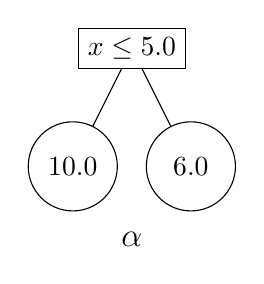
\begin{tikzpicture}
            \node[branch] {$x \le 5.0$}
             child {node[leaf] {10.0}}
             child {node[leaf] {6.0}};
         \node[font=\large, yshift=-1em] at (current bounding box.south) {$\alpha$};
        \end{tikzpicture}
        \quad
        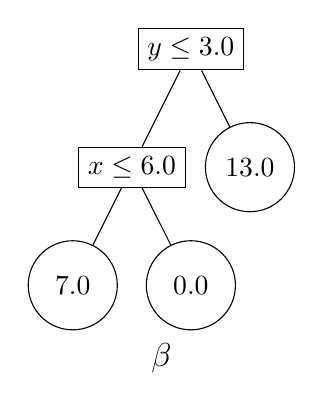
\begin{tikzpicture}
            \node[branch] {$y \le 3.0$}
             child {node[branch] {$x \le 6.0$}
                 child {node[leaf] {7.0}}
                 child {node[leaf] {0.0}}
             }
             child {node[leaf] {13.0}};
         \node[font=\large,yshift=-1em] at (current bounding box.south) {$\beta$};
        \end{tikzpicture}
        \quad
        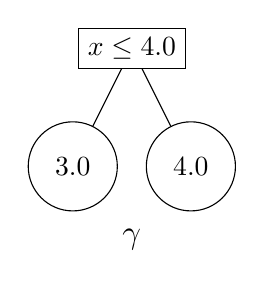
\begin{tikzpicture}
            \node[branch] {$x \le 4.0$}
             child {node[leaf] {3.0}}
             child {node[leaf] {4.0}};
         \node[font=\large,yshift=-1em] at (current bounding box.south) {$\gamma$};
        \end{tikzpicture}

    \caption{%
        A simple example of Q-trees for three actions, $\alpha$, $\beta$ and
        $\gamma$, and predicates on two variables, $x$ and $y$. Evaluating a
        state with $x=3$ and $y=5$, we would get Q-values 10.0, 13.0 and 3.0 for
        $\alpha$, $\beta$ and $\gamma$ respectively, meaning $\gamma$ would be
        the optimal action.
    }\label{fig:qTreeExample}
\end{figure}

The end result is a set of trees $\mathcal{T}$, one for each action $A \in
\mathcal{A}$, where any continuous valued state $S \in \mathcal{S}$ can be
evaluated to $Q^{\pi}_{S,A}$\todo{Should I ditch the $\pi$ superscript now?} in
any tree $T_A \in \mathcal{T}$ by following the path from the root node to a
leaf node as specified by the predicates in the branching nodes. That is, at
each branch node we follow the path to the `left' if the predicate is true for
$S$ and we follow the path to the `right' otherwise, untill we end up at a leaf
node which will then carry the value of $Q^{\pi}_{S,A}$. The subscript $A$ in
$T_A$ indicates that it is the tree specifying the Q-values of action $A$ and we
can now define $T_A(S): S, A \mapsto Q^{\pi}_{S,A}$. The greedy policy then just
have to choose a an action $A$ where $A = \argmin_{A \in \mathcal{A}}
T_A(S)$\footnote{Note that UPPAAL Stratego uses \textit{cost} rather than
\textit{reward}, therefore we minimize instead of maximizing}.

We propose to call these trees \textit{Q-trees} and provide a small example in
Figure~\ref{fig:qTreeExample}.



\section{Converging Q-trees to decision tree}%
\label{sec:convergeToDT}

A strategy represented by a set of Q-trees has a couple of disadvantages: first
of all, having to iterate all the trees and evaluate $S$ in each one of them
creates an amount of overhead\todo{I don't know}, and second, the structure of
the representation is not very intuitive to humans in the sense that the unique
evaluation of $S$ in each tree and the Q-values that they then return are very
hard to interpret.\todo{Maybe just cut this paragraph?}

We can convert the Q-trees into a single decision tree with actions --- not
Q-values --- in the leaf nodes so that the evaluation of $S$ in the tree yields
the optimal action for that state.

Let $\mathcal{V} = \{ V_1, V_2, \ldots, V_m \}$ be the set of all variables
(dimensions) in the state space. We then have that a state $S = {[v_1, v_2,
\ldots, v_m]}^{\tran}$ is a vector of instantiated values of each $V \in
\mathcal{V}$, ie. $V_i = v_i$. Following the path from the root node of any
Q-tree $T_A$ to a leaf node $L_i$, we can collect the constraints entailed by
each predicate in the branching nodes along the path to get a symbolic state
$S_i$ that represents an $m$-dimensional area (also called partition) of the
state space. The symbolic state is not given by concrete values of the
dimensions but rather by lower and upper bounds, that is $S_i = \{ (l_{1,i},
u_{1,i}), (l_{2,i}, u_{2,i}), \ldots, (l_{m,i}, u_{m,i}) \}$ where $l_{j,i}$ and
$u_{j,i}$ are the lower and upper bounds respectively of $V_j$ in the symbolic
state $S_i$ that the leaf $L_i$ entails.

With this, we can define a leaf in a Q-tree as $L_i = (S_i, q_a, A_i)$ where
$S_i$ is the symbolic state obtained from applying all the constraints on the
path to $L_i$, $A_i$ is the action pertaining to the tree that the leaf belongs
to and $q_{A_i}$ is the Q-value of action $A_i$ in all $S \in S_i$. The
algorithm for converting a set of Q-trees to a decision tree then starts by
gathering all these leaf triplets and sorting them in ascending order\footnote{%
    Again, UPPAAL Stratego computes for Q-values the expected \textit{cost}, so
the action with the lowest Q-value is the most preferable.} according to their
Q-value, and then pops the first leaf to create a root node and a path of
branching nodes until $S_1$ is fully specified. Then a decision leaf can be
inserted with label $A_1$, knowing that this is the optimal action for this
state. From here, we can continually pop and insert $L_2$, $L_2, \ldots, L_n$ in
that order, creating new branching nodes when needed and ignoring insertions
into areas that have already been covered by previous leafs (since the actions
of these will necessarily be more optimal than the later one because of inital
sorting).

The algorithm for this operation is given in Algorithm~\ref{}.


\section{Minimizing the decision tree}%
\label{sec:minimizingDT}

\lipsum[1]

\subsection{Empirical pruning}%
\label{subsec:empPruning}

\lipsum[2]

\subsection{Maximizing partition sizes}%
\label{subsec:findBoxes}

\lipsum[3]


\section{Rebuilding the tree}%
\label{sec:rebuildTree}

\lipsum[5]


\section{Experiments}%
\label{sec:experiments}

\subsection{Maximizing partitions}%
\label{subsec:experimentsMaxParts}

Continuing with the bouncing ball example, we now try and apply the
\texttt{MaxPartitions} algorithm (see Section~\ref{subsec:findBoxes}) to the
strategy trained by UPPAAL Stratego.  This first step is, as mentioned, to
convert the set of Q-trees into a decision tree. The reason for this is that is
one way to merge the (two) action specific partitionings of the state space into
one single partitioning where every area is prescribed one optimal action.

Due to the randomness involved in how the decision tree turns out (caused by the
fact that we randomize the order in which state bounds are turned into branching
nodes), we cannot expect excactly the same tree size at every instance of
performing the conversion. For this experiment, we did the conversion 100 times
and only saved the best (smallest) version of the tree. This gave us an instance
of the complete strategy represented by a tree with 86,807 paths from the root
to a leaf.

Since the bouncing ball example only has two state variables (position and
velocity) we can actually draw the state partitioning and colorize the different
partitions according to the action that is prescribed (green for no hit, red for
hit). This can be seen in Figure~\ref{fig:ballPartitioningBefore}.

\begin{figure}[ht]
    \centering
    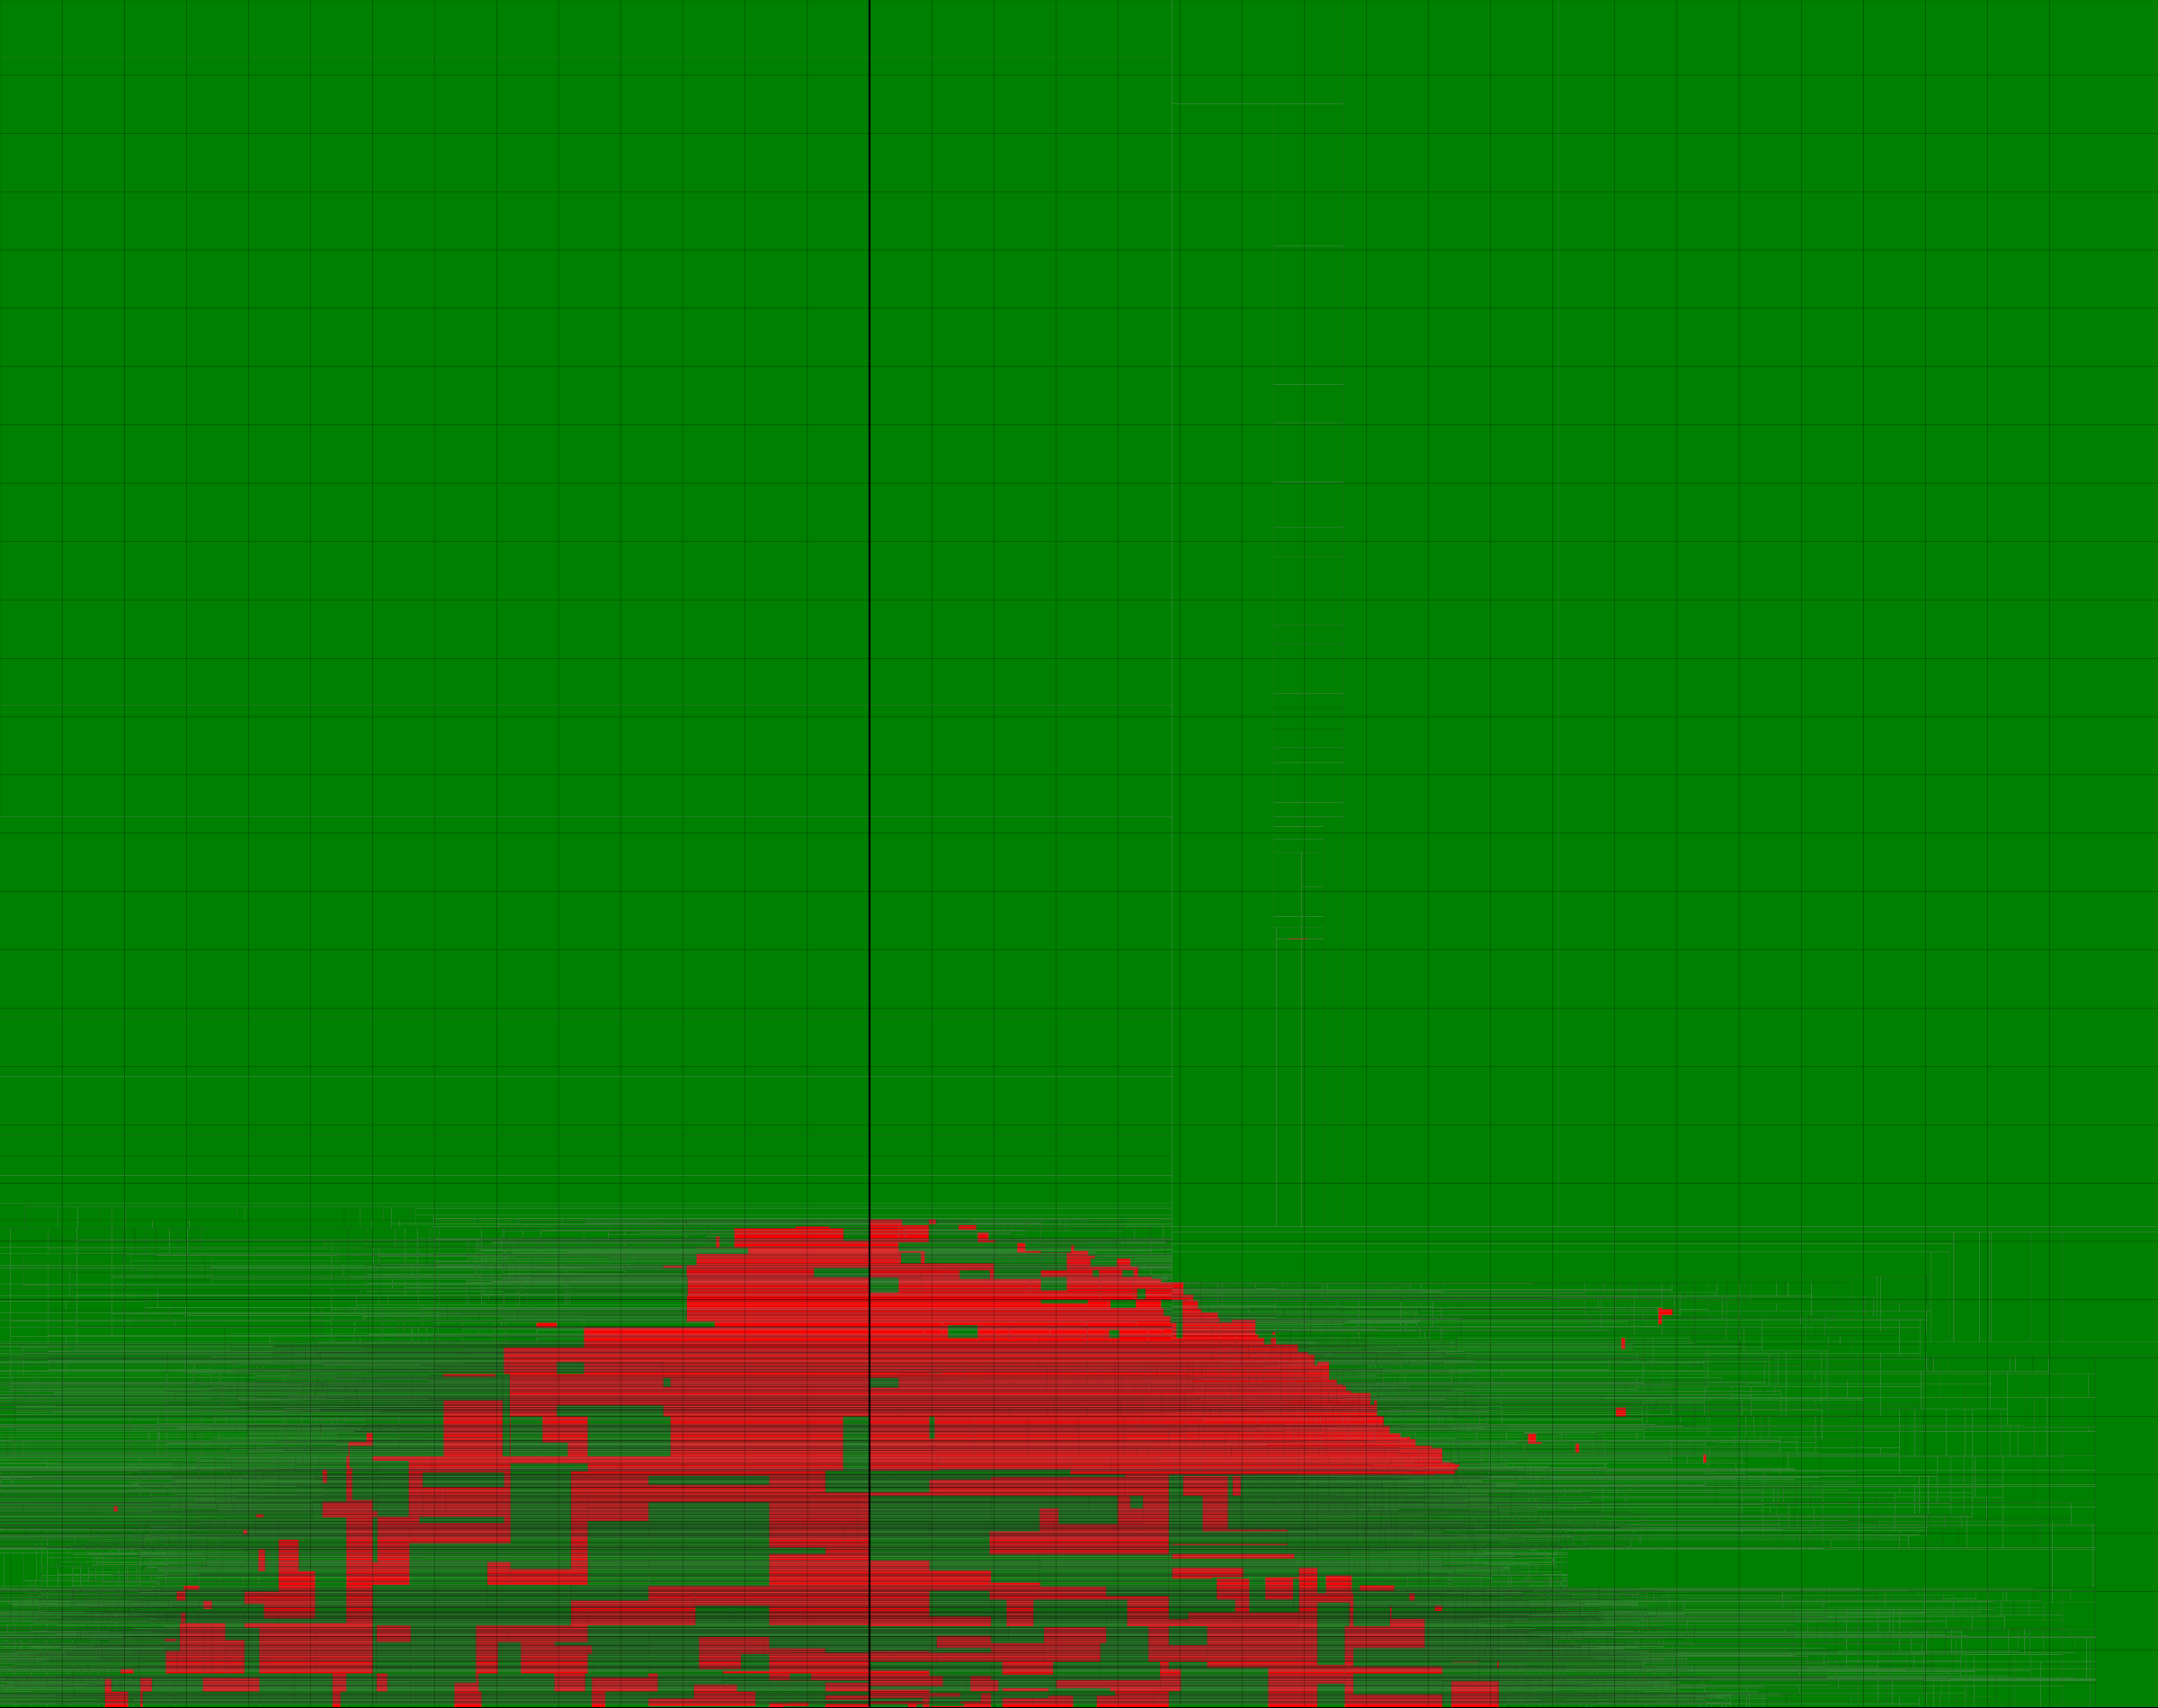
\includegraphics[width=0.8\textwidth]{ballPartitioningBefore}
    \caption{%
        A 2D visualization of the partitioning (dotted lines) of the state space
        of the bouncing ball model as it looks without any minimization
        attempts. The x-axis is velocity and the y-axis is the balls position.
        Green areas represents the action `no hit', red areas represents `hit'.
        The thick black line is $x=0$ and there have been drawn grid lines at
        every 1 tick.
    }\label{fig:ballPartitioningBefore}
\end{figure}

An inspection of this partitioning shows that a lot of partitions that are next
to each other share the same action which make them fit for combining, thus
reducing the overall number of partitions and maximizing the size of the
partitions. Using the \texttt{MaxPartitions} algorithm we obtain a new set of
partitions (not a DT yet) but the number has been dramatically reduced to only
703, that is, a 99.19\% reduction! The new partition can be seen in
Figure~\ref{fig:ballPartitioningAfter}.

\begin{figure}[h]
    \centering
    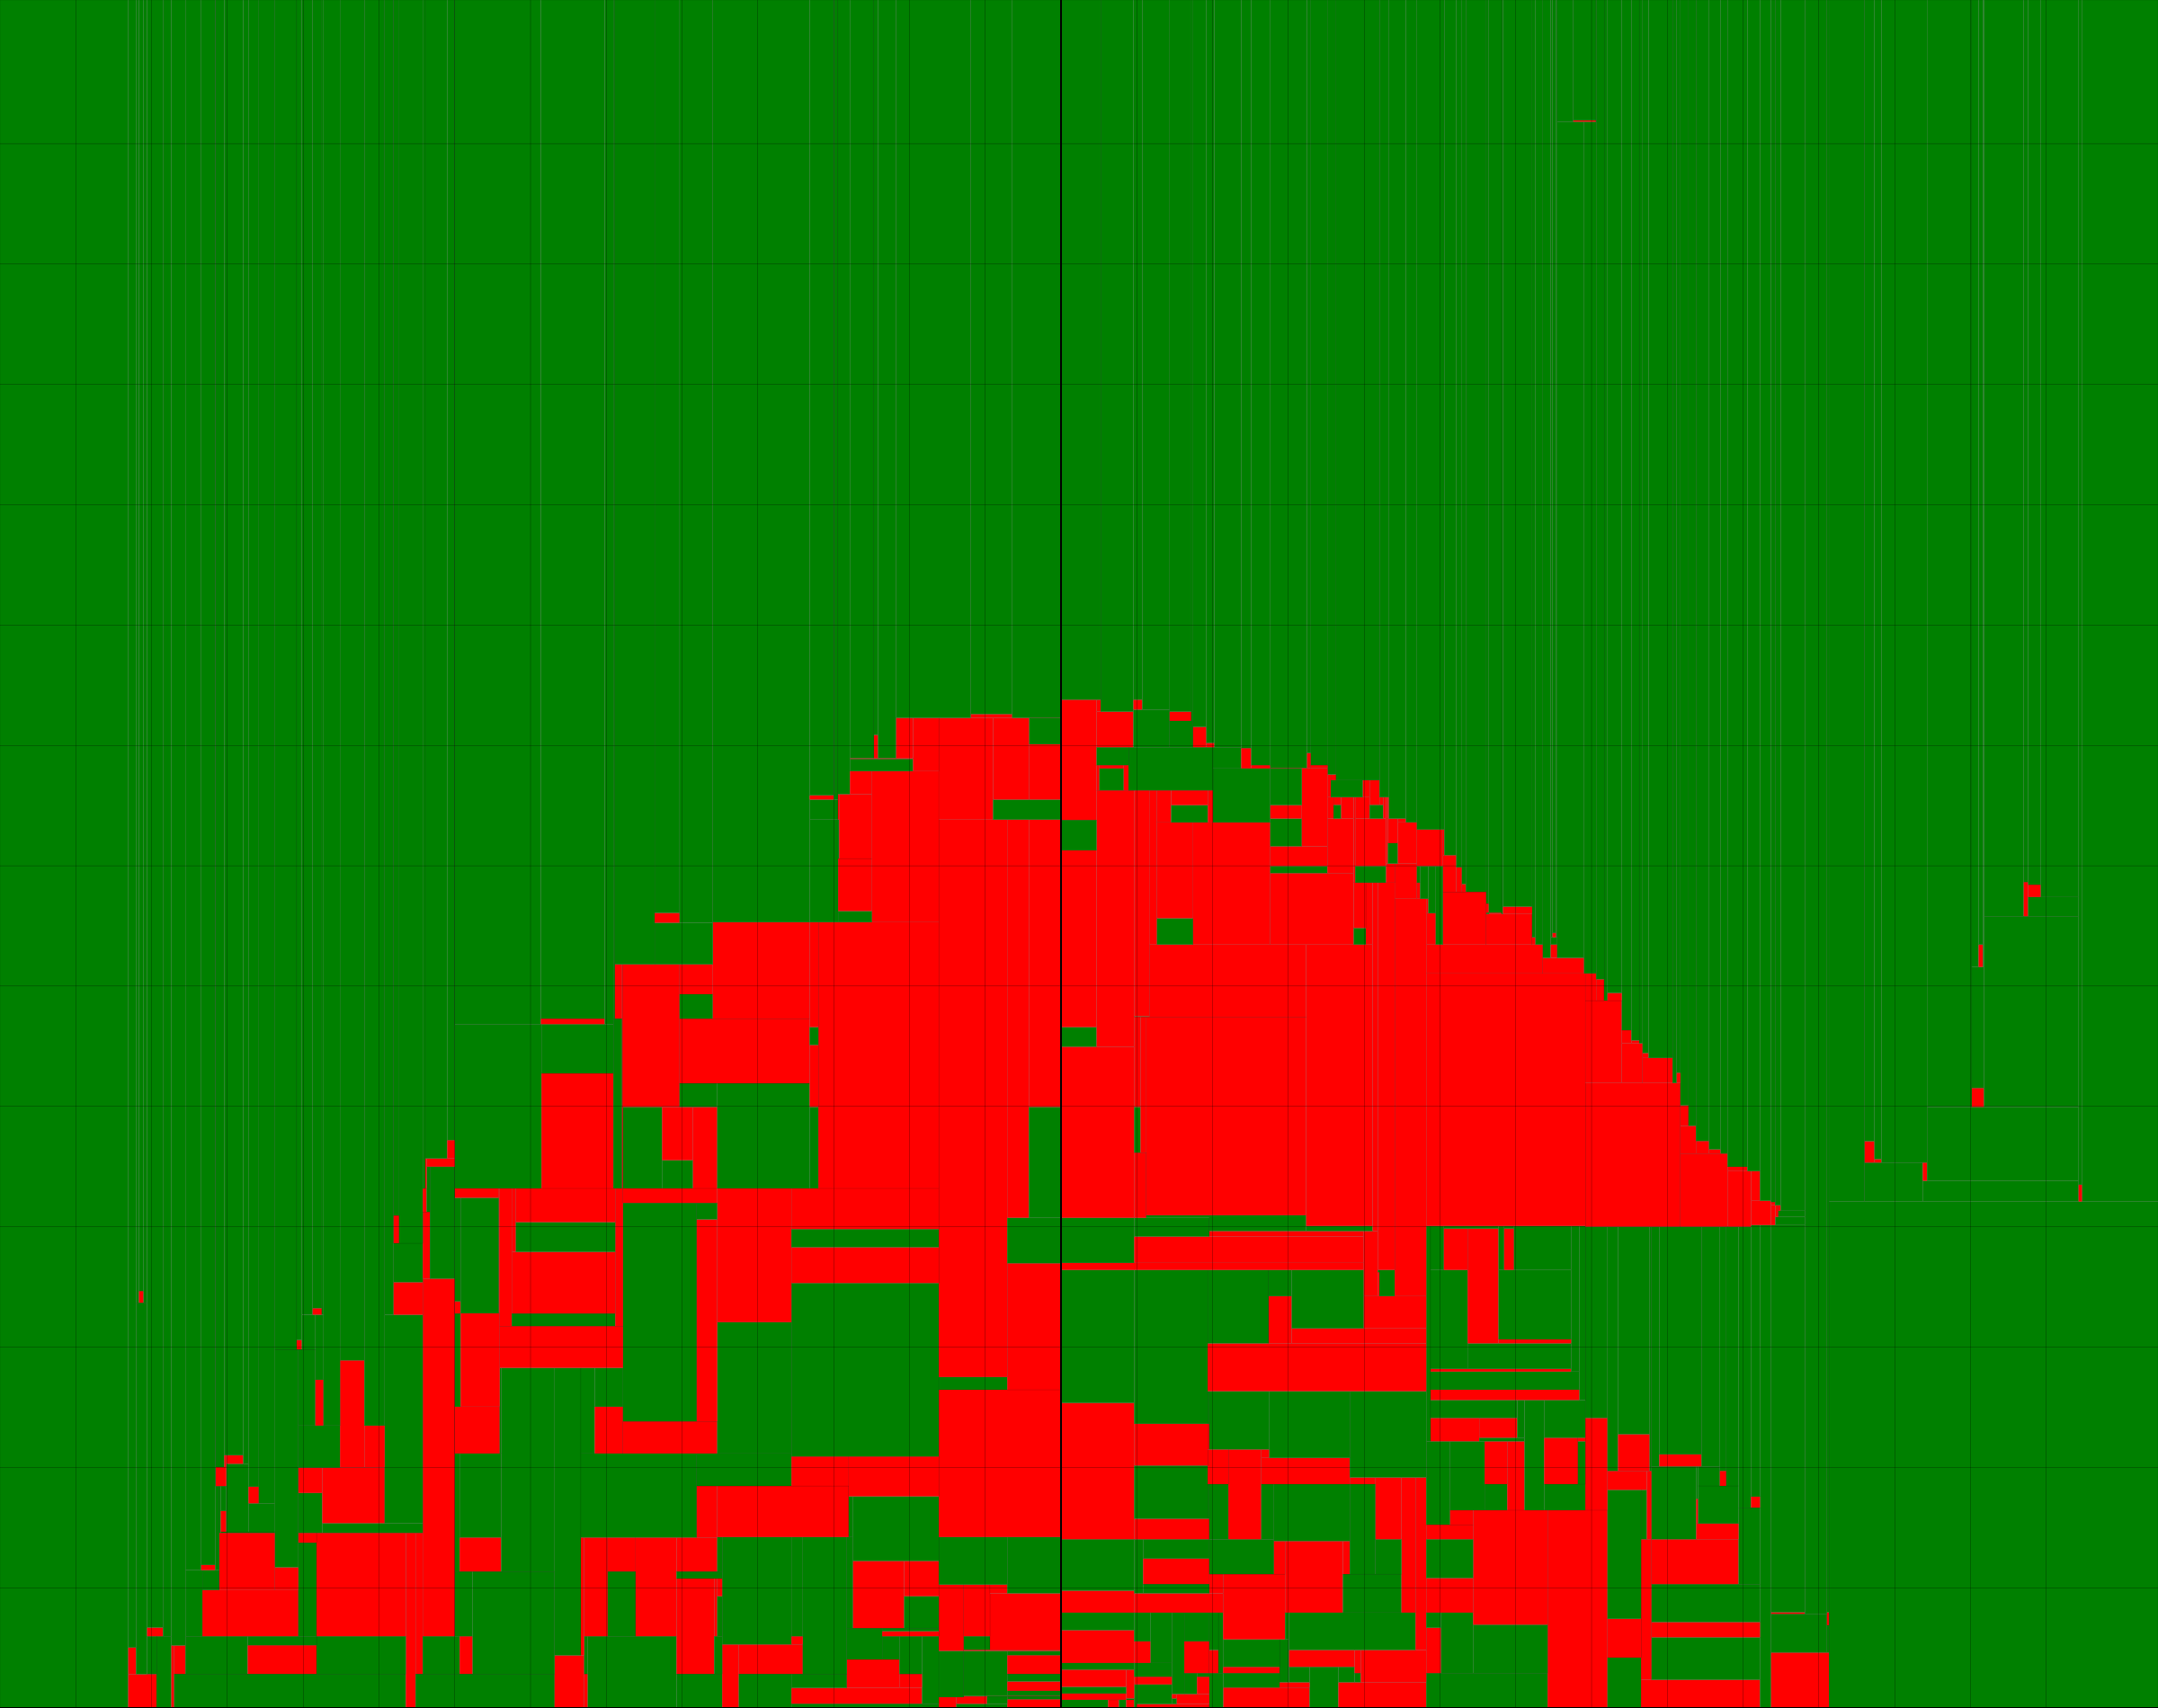
\includegraphics[width=0.8\textwidth]{ballPartitioningAfter}
    \caption{%
        A visualization of the same strategy as in
        Figure~\ref{fig:ballPartitioningBefore} but now with much fewer and
        larger partitions.
    }\label{fig:ballPartitioningAfter}
\end{figure}




\subsection{dtControl}%
\label{subsec:dtControl}

The tool \texttt{dtControl} has the ability to take a synthesized strategy
represented as a look-up table and convert the representation to a decision
tree that respects the safety requirements but compresses the size immensely.
This is naturally of great interest for our case, but both the Q-tree
representation and our own decision tree conversion alters the setup somewhat.

However, even though the tool actually supports directly working with the output
format of UPPAAL Stratego, this is only the case for strategies learned using
the \texttt{control[]} directive, which controls for certain defined safety
parameters to always be respected. In our case of the bouncing ball example, the
controller is trained with the \texttt{minE[]} directive, which minimizes a
given parameter (in this case, the number of times the controller hits the
ball).

Instead, we had to create our own output files to use as input for
\texttt{dtControl}. According to the documentation, a controller strategy can be
specified in a simple CSV format where each line contains an allowed
state/action pair, that is, $N$ values representing a state where the following
$M$ values constitutes an allowed action. For example, in the case of the
bouncing ball, we have two state variables (position and velocity) and one action
variable (hit or not hit), meaning each line would have three values.

We have attempted two experiments with different ways of specifying our original
controller.

In the first experiment, we used the trained controller to generate 30,000
samples of state/action pairs. That is, the UPPAAL model was run for 300
timesteps with the trained controller deciding what action to take in each
encountered state and then the state/action pairs were logged at each 0.01
timestep.

In the second experiment, we converted the strategy a set of Q-trees (the
initial UPPAAL format) to a DT as described in Section~\ref{sec:convergeToDT}.
This DT had a partition size (number of leaves/paths) of 91,054. We used these
partitions as the input data to \texttt{dtControl} by taking the maximum value
of each variable in each individual partition together with the optimal action
of that state. That is, we effectively specified the discretization of the state
space by defining the bounds of each state paired with the allowed/optimal
action.

\begin{table}[ht]
    \centering
    \caption{%
        Comparing the performance of controllers for the bouncing ball example
        over 1000 runs for 120 timesteps each before and after various attempts
        at minimizing the size through \texttt{dtControl}.  
    }\label{tab:dtcontrolTable}
    \begin{tabular}[t]{lccc}
        \toprule
        Version & Paths & Construction time & Expectation (hits) \\
        \midrule
        Original DT & 91,054 & --- & 38.431 \\
        Samples & 27,234 & 8:14 & 318.411 \\
        State bounds & 521 & 0:41 & 315.769 \\
        \bottomrule
    \end{tabular}
\end{table}


The results when applying the generated strategies to the model in UPPAAL are
given in Table~\ref{tab:dtcontrolTable} together with the baseline original
decision tree directly converted from the Q-tree set. As is seen, when we used
samples, we still got a somewhat large DT that took more than 8 minutes to
generate. And the perfomance (expected number of hits) is substantially worse
than the baseline version. For the version based on state bounds, we got a much
smaller tree with only 521 paths, but the performance was still very far from
the original.

\end{document}
